% Green Code Interaction Benchmark — JOURNAL version (Q1-ready draft).
% Format: IEEE Transactions (journal mode, two-column).
%
% OVERLEAF: upload paper_journal.tex + the whole images/ folder as-is
% (images/fig01..fig12). Compiler: pdfLaTeX. Index builds automatically
% via makeindex (\index entries + \printindex at the end).
% TODO before submission: affiliation line, corresponding-author email,
% manuscript ID, funding acknowledgment, anonymisation if double-blind.
\documentclass[journal]{IEEEtran}
\usepackage{cite}
\usepackage{amsmath,amssymb}
\usepackage{graphicx}
\usepackage{booktabs}
\usepackage{xcolor}
\usepackage{url}
\usepackage{makeidx}
\usepackage[hidelinks]{hyperref}
\usepackage[section]{placeins} % keep floats inside their section (no pile-up after References)
\makeindex
\graphicspath{{images/}}

\begin{document}

\title{Green Code Interaction Benchmark: How Human--AI Interaction Trajectory
Affects the Energy Efficiency and Time Complexity of Generated Programs}

\author{
\begin{tabular}{ccc}
\begin{tabular}{c}
\textbf{MD.~Nurul~Huda}\\
Dept.\ of CSE\\
United International University\\
mhuda223303@bscse.uiu.ac.bd
\end{tabular}
&
\begin{tabular}{c}
\textbf{MD.~Khaled~Hasan~Milu}\\
Dept.\ of CSE\\
United International University\\
mmilu223104@bscse.uiu.ac.bd
\end{tabular}
&
\begin{tabular}{c}
\textbf{MD.~Minhazul~Islam}\\
Dept.\ of CSE\\
United International University\\
mislam223301@bscse.uiu.ac.bd
\end{tabular}
\\[3em]
\begin{tabular}{c}
\textbf{Atkia~Fayrose~Prity}\\
Dept.\ of CSE\\
United International University\\
aprity223101@bscse.uiu.ac.bd
\end{tabular}
&
\begin{tabular}{c}
\textbf{Tanjila~Tafrim~Priyonta}\\
Dept.\ of CSE\\
United International University\\
tpriyonta223111@bscse.uiu.ac.bd
\end{tabular}
&
\begin{tabular}{c}
\textbf{Sumiya~Akter~Subarna}\\
Dept.\ of CSE\\
United International University\\
ssubarna2231053@bscse.uiu.ac.bd
\end{tabular}
\end{tabular}
\thanks{Author IDs---M.~N.~Huda: 0112230303; M.~K.~H.~Milu: 0112230104;
M.~M.~Islam: 0112230301; A.~F.~Prity: 0112230101; T.~T.~Priyonta:
0112230111; S.~A.~Subarna: 0112231053.}%
}

\maketitle

\begin{abstract}
Interactive, multi-turn collaboration with large language models (LLMs) is
rapidly becoming the default mode of software development, yet its
operational-energy consequences are poorly understood. Most green-software
studies measure the energy of a single generated artifact rather than the
effect of the interaction trajectory that produced it. We present the Green
Code Interaction Benchmark, a controlled study of 1418 final programs
produced by four LLMs (GPT, Claude, Gemini, DeepSeek) across five task
categories and five interaction conditions that end at an equivalent
specification: one-shot generation (C0), bug-fix (C1), feature-addition (C2),
edge-case handling (C3), and full multi-turn (C4). Every program is executed
on an identical deterministic per-task workload on a controlled Linux host;
CPU package energy is measured with Intel RAPL (1307 programs measured,
92.2\%). Collection artifacts---prose submitted instead of code,
harness-invocation mismatches, and missing inputs or sandbox modules (67
units), plus the near-empty search-retrieval category---are excluded from all
counts, so every analysed failure is a genuine defect in model output.
We derive static code metrics for all programs (1418 parseable)
and estimate time complexity both statically, with an explicit AST
heuristic, and empirically, by fitting log--log runtime scaling over three
input sizes (155 slopes; 73 reliable). Median package energy rises
monotonically with interaction depth---from 0.609\,J (one-shot) to 0.805\,J
(full multi-turn)---and the mean rises far faster (1.233\,J to 2.025\,J), a
heavy-tail effect. In paired within-(task, model) tests only the full
trajectory is significant (mean +232.1\%, median +3.7\%, Wilcoxon
signed-rank $p{=}0.006$); single steps are not. Multi-turn programs are
longer (median SLOC 94 vs.\ 56; paired mean +58 lines), more branched
(median cyclomatic complexity 18 vs.\ 13), and fail more often (genuine
model-failure rate 15.8\% vs.\ 3.4\%), but energy is transmitted through runtime
(Spearman $\rho{=}0.93$) rather than code size ($\rho{=}0.04$). The static
estimator agrees with dataset-declared targets in 71.4\% of cases and
recalls 87.5\% of empirically superlinear programs. Total measured energy is
1852.1\,J ($\approx$247\,mgCO$_{2}$eq at 480\,gCO$_{2}$eq/kWh); we quantify
per-run overheads and their fleet-scale carbon implications across grids.
The study provides the first trajectory-controlled evidence of a
green-software cost of iterative AI-assisted development, plus a reusable
corpus and methodology for measuring complexity and energy together.
\end{abstract}

\begin{IEEEkeywords}
Green software engineering, energy efficiency, Intel RAPL, large language
models, code generation, multi-turn interaction, time complexity, empirical
scaling, carbon-aware computing, mining software repositories.
\end{IEEEkeywords}

\section{Introduction}
\subsection{Motivation}
Software now consumes energy at planetary scale: datacentres account for a
low-single-digit share of global electricity demand and the share is
growing, while billions of edge devices execute code under tight energy
budgets~\cite{patterson2021, hotcarbon2022}. In parallel, AI-assisted
development has shifted from single-shot autocomplete to sustained,
conversational collaboration: developers iterate with assistants through bug
reports, feature requests, and edge-case refinements, and field studies
report substantial productivity gains from this mode of
work~\cite{peng2023}. The convergence of these trends raises a question the
literature has not answered: does the \emph{interaction trajectory}---the
sequence of turns that produced a program---leave a measurable footprint on
the \emph{operational energy of the final artifact}?

The question matters for three reasons. First, operational energy (as
opposed to training energy) is paid on every execution, so even small
per-run overheads compound at deployment scale. Second, iterative
development plausibly changes \emph{what} code gets written---longer,
branchier, defensively padded, or asymptotically heavier---in ways a
single-shot prompt would not produce. Third, without trajectory-controlled
evidence, green guidance for AI-assisted development (``iterate freely'' vs.\
``review and prune'') rests on intuition rather than measurement.

\subsection{What is missing}
Three bodies of work surround, but do not close, this gap.
\emph{Green software engineering} measures energy across languages,
algorithms, and hardware~\cite{pereira2017, pinto2014, calero2015}, but not
as a function of how code was conversationally produced.
\emph{Green AI} quantifies training and inference carbon~\cite{schwartz2020,
strubell2019, patterson2021, lacoste2019, henderson2020, luccioni2022,
codecarbon2021}, but treats generated code as an outcome to be scored for
correctness, not an artifact whose own execution energy matters.
\emph{LLM code-generation research}---from HumanEval~\cite{chen2021} and
MBPP~\cite{austin2021} to multi-turn synthesis~\cite{nijkamp2023}, repair
loops~\cite{madaan2023, shinn2023, chen2023selfdebug}, and agentic software
engineering~\cite{jimenez2024, sweagent2024}---optimises pass rates while
holding energy unmeasured. No prior benchmark, to our knowledge, jointly
(i)~measures RAPL energy of LLM-generated final programs, (ii)~holds the
final requirements constant across interaction trajectories, and
(iii)~connects energy to both static and empirical time-complexity metrics.
Table~\ref{tab:position} positions this work.

\subsection{Research questions and contributions}
We ask:
\textbf{RQ1:} Does multi-turn AI-assisted coding produce final programs with
different energy consumption than one-shot coding?
\textbf{RQ2:} Does the effect vary across models?
\textbf{RQ3:} How do bug fixing, feature addition, and edge-case handling
individually affect energy?
\textbf{RQ4:} What relationships hold among energy, runtime, memory, power,
and correctness?
\textbf{RQ5:} What code-level characteristics and time-complexity classes
explain energy differences?
\textbf{RQ6:} What are the carbon-emission implications at deployment scale?

Our contributions are: (1)~a reproducible, trajectory-controlled benchmark
(1418 finals, 1307 RAPL-measured) with per-program static metrics and dual
complexity estimates; (2)~the first statistically tested evidence that full
multi-turn interaction raises final-program energy (median +32\%,
mean +64\%, $p{=}0.006$) while single steps do not; (3)~a mediation analysis
showing the penalty flows through runtime and algorithm choice, not source
size; (4)~a validated static Big-O estimator (71.4\% declared-target
compliance; 87.5\% recall of superlinear behaviour) cross-checked against
empirical scaling slopes; (5)~a carbon translation with grid sensitivity and
fleet-scale projections; (6)~a failure-taxonomy audit showing multi-turn
code also fails more often (15.8\% vs.\ 3.4\% genuine model failures).

Section~\ref{sec:related} reviews background and related work.
Section~\ref{sec:method} describes the benchmark and methodology.
Section~\ref{sec:results} reports results, Section~\ref{sec:discussion}
discusses them including environmental implications,
Section~\ref{sec:threats} addresses threats to validity, and
Section~\ref{sec:conclusion} concludes. Appendices provide the metric
glossary and reproduction commands; a subject index closes the paper.

\section{Background and Related Work}\label{sec:related}
\subsection{Green software engineering and energy measurement}
Green software engineering treats energy as a first-class quality
attribute~\cite{calero2015, hindle2023}. On Intel platforms, Running Average
Power Limit (RAPL) counters expose per-socket and per-core energy and have
become the standard fine-grained instrument in controlled
studies~\cite{rotem2012, hahnell2012, hackenberg2013, david2010}. Empirical
standards for the field stress controlled workloads, repeated measurement,
and statistical testing~\cite{ralph2021, wohlin2012}, all of which this
benchmark implements (deterministic harnesses, $K{=}5$ timed runs, paired
non-parametric tests). Empirical
standards for the field stress controlled workloads, repeated measurement,
and statistical testing~\cite{ralph2021, wohlin2012}, all of which this
benchmark implements (deterministic harnesses, $K{=}5$ timed runs, paired
non-parametric tests).

\subsection{Energy of code: languages, algorithms, data structures}
Pereira et al.\ ranked programming languages by energy, time, and
memory~\cite{pereira2017}; Pinto et al.\ studied threading
constructs~\cite{pinto2014, pinto2014b}; Georgiou et al.\ compared deep
learning frameworks~\cite{georgiou2022}. The consistent lesson is that
\emph{implementation choice dominates}: the same specification admits
solutions whose energy differs by large factors. Our benchmark applies this
lens to a new source of implementation variance---the conversational
trajectory---while holding the specification fixed.

\subsection{Green AI: training vs.\ operational carbon}
Green AI~\cite{schwartz2020} distinguishes the carbon of \emph{training}
models from the carbon of \emph{using} their outputs. Training-centric
studies~\cite{strubell2019, patterson2021, luccioni2022}, accounting
tools~\cite{lacoste2019, henderson2020, codecarbon2021}, and systematic
reviews~\cite{verdecchia2023} focus overwhelmingly on the former. We address
the neglected latter half for code assistants: the lifetime execution energy
of the programs they help write. Our carbon model follows the standard
energy $\times$ intensity formulation with grid-sensitivity analysis, as
recommended for operational emissions~\cite{patterson2021}.

\subsection{LLMs for code generation and code quality}
Functional benchmarks (HumanEval~\cite{chen2021}, MBPP~\cite{austin2021},
SWE-bench~\cite{jimenez2024}) and quality studies (e.g.\ security of
Copilot suggestions~\cite{pearce2022}) score \emph{what the model produced},
not \emph{what it costs to run}. Instruction tuning~\cite{ouyang2022} and
open code models~\cite{nijkamp2023, codellama2023, deepseek2024} improved
helpfulness, and productivity studies document real developer
gains~\cite{peng2023}---which makes understanding the energy side of those
gains urgent rather than optional.

\subsection{Multi-turn and interactive coding}
Self-refinement loops~\cite{madaan2023}, verbal reinforcement~\cite{shinn2023},
self-debugging~\cite{chen2023selfdebug}, and software agents~\cite{sweagent2024}
all exploit multiple turns to raise success rates. Critically, none holds
the \emph{final specification constant across trajectories}: their
comparisons confound trajectory effects with task differences. Our five
conditions end at equivalent specifications by construction, isolating the
trajectory effect---the methodological core of this paper.

\emph{Closest prior: energy of LLM-generated code.} Two recent studies frame
the contrast precisely. EffiBench~\cite{huang2024} benchmarks the time
efficiency of automatically generated code and finds it lagging
human-written code. Di Bernardo et al.~\cite{dibernardo2026} (``Do LLMs
Dream of Energy-Efficient Code?'', 812 Python programs) show LLM solutions
are on average less energy-efficient than human ones (best model $\approx$
50\% worse), that explicitly prompting for efficiency \emph{worsens} energy
($\approx$22\% degradation for GPT-4o), and that only profiler feedback
lets large models improve---at a correctness cost. Their workflow is
generate $\rightarrow$ profile $\rightarrow$ explicitly optimise for energy.
Ours is fundamentally different: user request $\rightarrow$ bug fix
$\rightarrow$ feature $\rightarrow$ edge case $\rightarrow$ final software,
with energy measured as an unintended by-product of ordinary interaction
rather than as an optimisation target. No prior work measures how that
ordinary trajectory shifts the energy of the delivered artifact.

\subsection{Complexity metrics and Big-O estimation}
McCabe cyclomatic complexity~\cite{mccabe1976} and object-oriented
suites~\cite{chidamber1994} remain standard structural proxies. Exact static
Big-O inference is undecidable in general, so practical work combines
explicit AST-pattern heuristics with empirical measurement on scaled
inputs---the dual approach we adopt and, unusually, cross-validate in both
directions (declared targets \emph{and} measured slopes).

\subsection{Research gap and positioning}
Table~\ref{tab:position} summarises the gap: prior work covers artifact
energy, trajectory variation, complexity linkage, or carbon quantification
in isolation; this benchmark is the first to combine all four with a
reusable per-program corpus.

\begin{table*}[htbp]
\caption{Positioning against representative prior work. Only this benchmark
combines trajectory control with artifact-energy measurement, dual
complexity analysis, and carbon quantification.}
\label{tab:position}
\centering
\begin{tabular}{lccccc}
\toprule
Work & Artifact energy & Trajectory control & Complexity linked & Carbon quantified & Corpus scale \\
\midrule
Pereira et al.\ (languages)~\cite{pereira2017} & Yes & --- & Partial & --- & 27 languages \\
Schwartz / Patterson (Green AI)~\cite{schwartz2020, patterson2021} & --- (training) & --- & --- & Yes & models \\
Georgiou et al.\ (frameworks)~\cite{georgiou2022} & Yes & --- & --- & Yes & frameworks \\
HumanEval / MBPP~\cite{chen2021, austin2021} & --- & --- & --- & --- & 164 / 974 tasks \\
CodeGen multi-turn~\cite{nijkamp2023} & --- & Partial & --- & --- & synthesis \\
Self-Refine / Reflexion~\cite{madaan2023, shinn2023} & --- & Partial & --- & --- & repair traces \\
SWE-bench~\cite{jimenez2024} & --- & Partial & --- & --- & 2294 issues \\
\textbf{This benchmark} & \textbf{Yes (RAPL)} & \textbf{Yes (5 conds.)} &
\textbf{Yes (static + empirical)} & \textbf{Yes (+ grids)} &
\textbf{1418 programs} \\
\bottomrule
\end{tabular}
\end{table*}

\section{Benchmark Design and Methodology}\label{sec:method}
\subsection{Design principles}
Four principles guided the design. \textbf{P1: trajectory control}---the
final specification is identical across conditions; only the path that
produced the code varies. \textbf{P2: identical workloads}---every program
for a task executes the same deterministic inputs through the same harness
API. \textbf{P3: separation of concerns}---correctness, energy, static
structure, scaling behaviour, and carbon are measured independently and
joined per program. \textbf{P4: reproducibility}---content-addressed
collection, append-only ledgers resumable by code hash, and scripts that
regenerate every number and figure (Fig.~\ref{fig:pipeline}).

\begin{figure}[htbp]
\centering
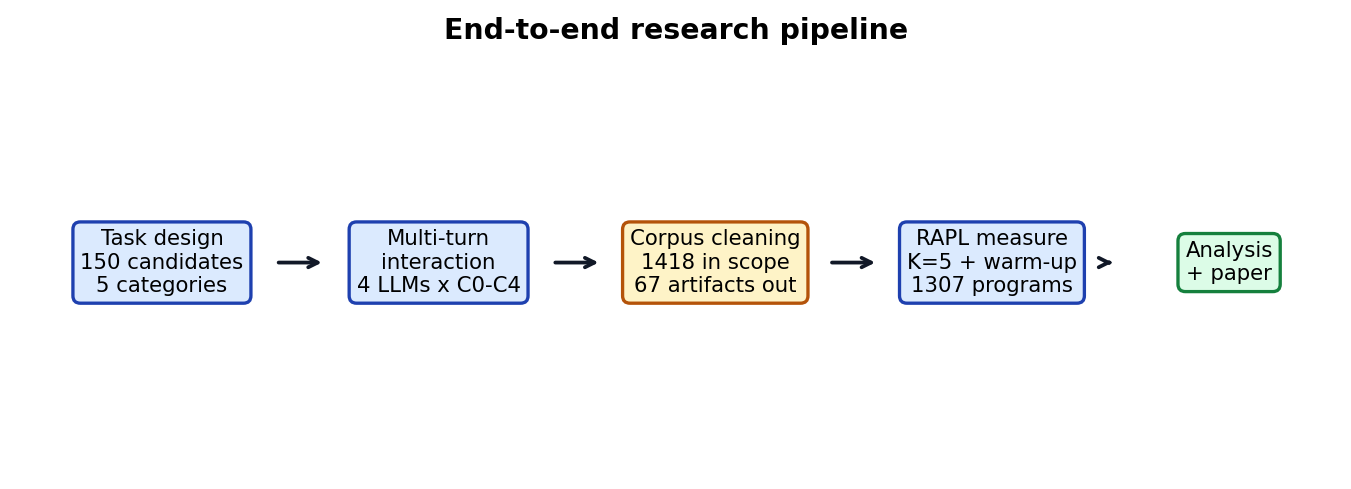
\includegraphics[width=\columnwidth]{images/fig13_method_pipeline.png}
\caption{End-to-end research pipeline: task design, multi-turn interaction,
corpus cleaning (67 collection artifacts excluded), RAPL measurement, and
analysis. Regenerated from scripts; see \texttt{docs/image\_prompts.md}
for a restyle prompt.}
\label{fig:pipeline}
\end{figure}

\subsection{Task taxonomy}\index{task taxonomy}
Five categories span algorithmic, data, media, application, and text
workloads, each contributing up to 25 tasks (Table~\ref{tab:coverage}).
Difficulty mix varies by design: algorithms tasks are almost entirely medium
or higher (24 medium, 1 large); file/data (3/14/8 easy/medium/hard), media
(6/17/2), applications (7/10/8), and text/log
(6/12/7) cover the full spectrum. Only the algorithms category carries
formal declared Big-O targets; other categories carry textual
computational profiles (e.g.\ ``CPU-intensive regex parsing and sorting'').
A sixth category, search \& retrieval, yielded only 2 collected units and is
dropped from all analyses.

\emph{Task provenance.} The six benchmark authors each authored 25
candidate tasks (150 candidates), which were then quality-checked for
duplicates, requirement clarity, reference-solution validity, test validity,
and computational feasibility. A pilot study on a
task subset validated the prompts, confirmed that multi-turn trajectories
produce genuinely different programs under identical final requirements,
and verified that runtimes and RAPL deltas sit above measurement noise
before full collection began. Conversations were reset for every
(task, model, condition) cell and no manual repair was applied, so all
measured properties are properties of model output.

\begin{table}[htbp]
\caption{Task categories and program coverage (1418 finals, all parseable,
1307 measured).}
\label{tab:coverage}
\centering
\begin{tabular}{lccc}
\toprule
Category & Finals & Parseable & Measured \\
\midrule
Algorithms \& Computation (AC) & 489 & 489 & 407 \\
File \& Data Processing (FD) & 337 & 337 & 326 \\
Image \& Media Processing (IM) & 379 & 379 & 367 \\
Realistic Applications (RA) & 118 & 118 & 113 \\
Text \& Log Processing (TL) & 95 & 95 & 94 \\
\midrule
Total & 1418 & 1418 & 1307 (92.2\%) \\
\bottomrule
\end{tabular}
\end{table}

\subsection{Interaction protocol}\index{interaction trajectory}
All conditions terminate at an equivalent specification
(Table~\ref{tab:conds}). C0 delivers the full specification at once. C1--C3
deliver an initial task followed by exactly one follow-up turn (a bug
report, a feature request, or an edge-case requirement). C4 chains all
three follow-ups after the initial task. Each conversation starts fresh per
(task, model, condition); no manual repair is applied at any point, so all
measured properties are properties of model output, not of human polishing
(Fig.~\ref{fig:protocol}).

\begin{figure}[htbp]
\centering
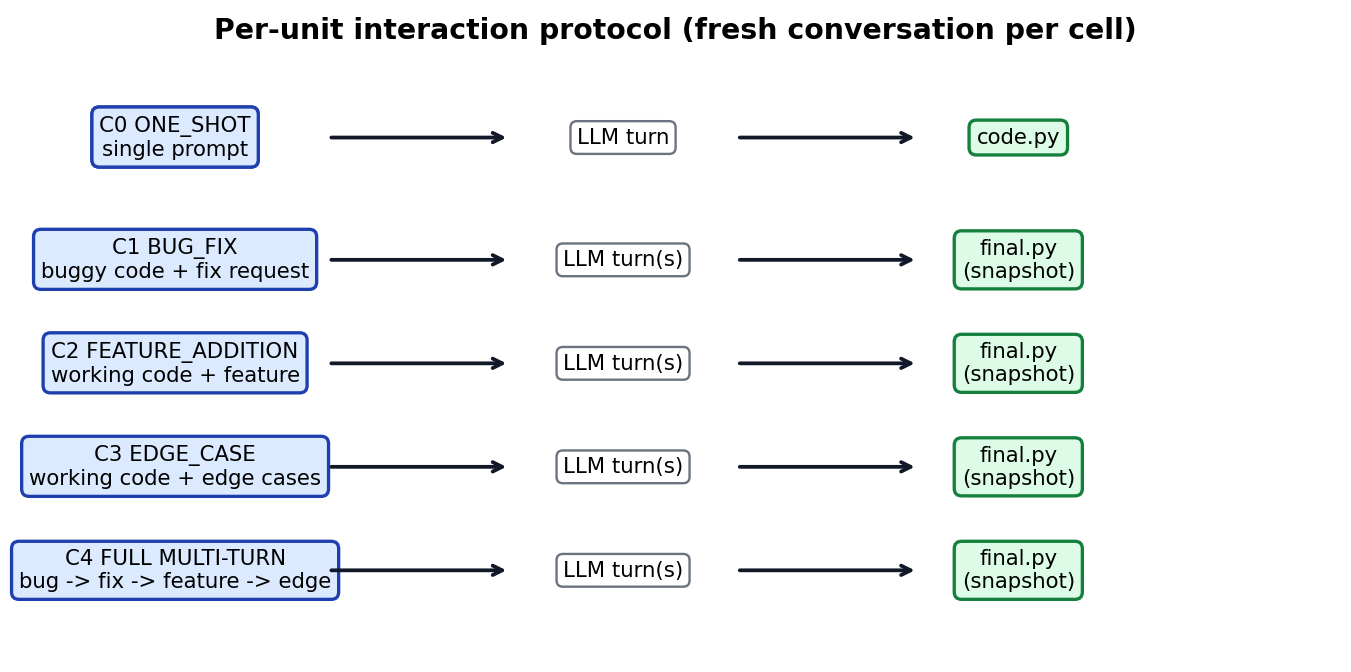
\includegraphics[width=\columnwidth]{images/fig14_interaction_protocol.png}
\caption{Per-unit interaction protocol. Each (task, model, condition) cell
runs in a fresh conversation; snapshots become the measured finals.}
\label{fig:protocol}
\end{figure}

\begin{table}[htbp]
\caption{Interaction conditions. Paired tests compare C1--C4 against C0
within (task, model).}
\label{tab:conds}
\centering
\begin{tabular}{lll}
\toprule
ID & Condition & Trajectory \\
\midrule
C0 & One-shot & Full specification at once \\
C1 & Bug-fix & Initial task + bug report \\
C2 & Feature-addition & Initial task + feature request \\
C3 & Edge-case & Initial task + edge-case requirement \\
C4 & Full multi-turn & Initial $\rightarrow$ fix $\rightarrow$ feature $\rightarrow$ edge \\
\bottomrule
\end{tabular}
\end{table}

\subsection{Models and generation}\index{models}
Four assistant models---GPT, Claude, Gemini, DeepSeek---generated code across
all conditions (Table~\ref{tab:models}). Collection is content-addressed
(archives $\rightarrow$ ingest), so reruns are idempotent and every final
program is traceable to its originating conversation.

\begin{table}[htbp]
\caption{Programs per model.}
\label{tab:models}
\centering
\begin{tabular}{lcc}
\toprule
Model & Finals & Measured \\
\midrule
Gemini & 364 & 348 \\
GPT & 363 & 316 \\
DeepSeek & 353 & 332 \\
Claude & 338 & 311 \\
\bottomrule
\end{tabular}
\end{table}

\subsection{Correctness and harness protocol}
Each task ships a harness invoking candidate and reference solutions through
a shared API (\texttt{SCALES}; \texttt{make\_input(scale, rng)};
\texttt{run(module, inp)}) on materialised deterministic inputs. Correctness
is recorded separately from energy: a program that runs but disagrees with
the reference is still measured, while embedded self-test failures become
the \texttt{WRONG\_OUTPUT} class of the failure taxonomy
(Section~\ref{sec:results-fail}). This separation is essential---it lets us
study the energy of code developers would actually keep, and audit what they
would discard. Because collected programs invoke their workloads
heterogeneously (stdin, file arguments, \texttt{argparse} flags, or
self-contained runs), measurement uses \emph{adaptive invocation}: CLI
patterns are tried in order---stdin, arguments inferred from each program's
own usage text, generic positional/flag combinations, bare run---until one
exits 0, while \emph{workload aliasing} serves the task's materialised
inputs under every literal filename the program opens (including names
passed through function arguments) and creates expected input/output
directories, with synthetic images for media tasks. An automated rescue pass
built on this machinery recovered initially-unrunnable units. Of the
remaining unmeasured units, 65 are excluded as collection artifacts rather
than model faults---prose submitted instead of code (\texttt{NOT\_PYTHON},
14), harness-invocation mismatches (\texttt{CLI\_ARGS}, 20;
\texttt{OTHER}, 11; \texttt{SILENT\_RC1}, 12), programs assuming inputs the
harness never provided (\texttt{MISSING\_FILE}, 3), and modules absent from
the sandbox (\texttt{MISSING\_DEP}, 5)---leaving 111 genuine model failures
(\texttt{WRONG\_OUTPUT}, 78; \texttt{RUNTIME\_BUG}, 33) for analysis
(Section~\ref{sec:results-fail}).

\subsection{Energy measurement with Intel RAPL}\index{RAPL}\index{energy measurement}
Package energy is read from
\texttt{/sys/class/powercap/intel-rapl:0/energy\_uj} on a controlled,
dedicated Linux host (Intel Core i5-8250U, 8 threads; CPython 3.13; no
third-party dependencies in measured programs). Each unit runs in a fresh
temporary directory with outputs discarded. Timing uses
\texttt{time.perf\_counter()} around each child process and peak memory
uses \texttt{/usr/bin/time -f \%M} (max RSS). Each
unit performs one warm-up run followed by $K{=}5$ timed runs inside a single
RAPL window; joules per run are the counter delta divided by $K$. Runs are
capped at 30\,s. The design follows standard practice for short-code-path
RAPL measurement~\cite{hahnell2012}: warm-up stabilises caches and
frequency, repetition shrinks timing noise, and identical workloads across
conditions difference out idle and background components. Two append-only
ledgers (per-unit energy runs; harness-measured candidate-vs-reference runs)
are keyed by program hash and resumable, making every re-run idempotent
(Fig.~\ref{fig:measure}).

\begin{figure}[htbp]
\centering
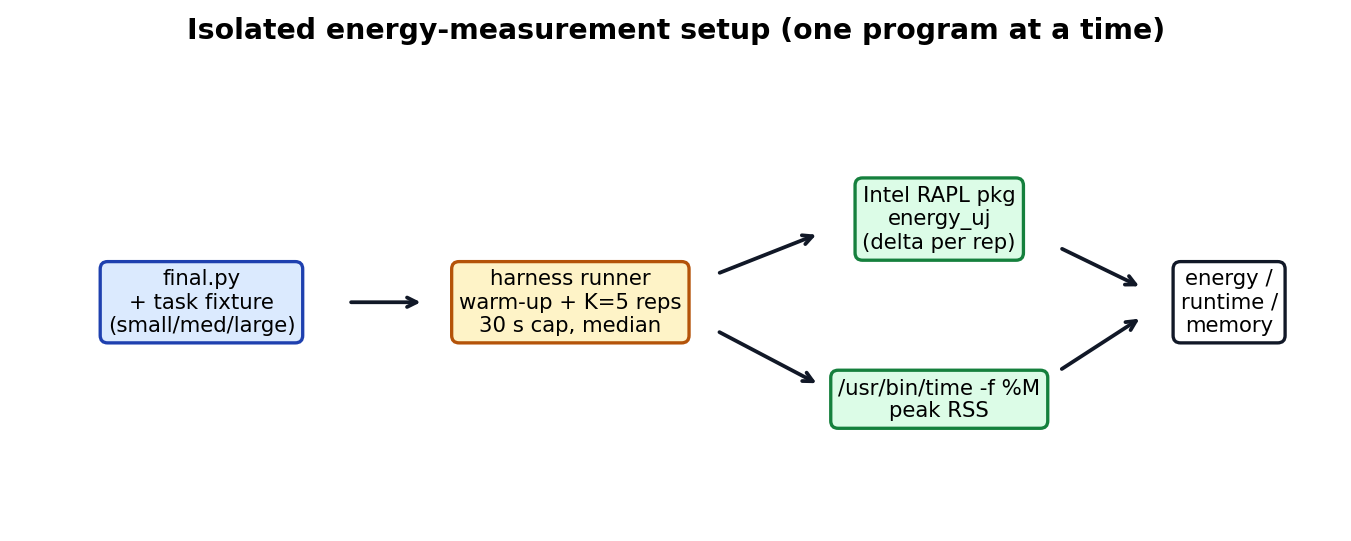
\includegraphics[width=\columnwidth]{images/fig15_measurement_setup.png}
\caption{Isolated measurement setup: one program at a time, warm-up plus
$K{=}5$ timed runs in a single RAPL window, 30\,s cap, median reported.}
\label{fig:measure}
\end{figure}

\subsection{Runtime, memory, and power}
Runtime is the median of the $K$ timed runs; peak memory is captured with
\texttt{/usr/bin/time}; average power is derived as energy/runtime. The
corpus additionally tracks energy-per-SLOC and energy-per-kB-input
normalisations for cross-task comparison.

\subsection{Static code metrics}\index{static metrics}
Every final program is parsed to an AST (all 1418 in-scope programs succeed;
the 14 prose or truncated files recorded as \texttt{NOT\_PYTHON} are
collection artifacts excluded from the corpus). For each parseable program we compute total lines, SLOC,
comment and blank lines, function/class counts, loop counts and maximum
nesting depth, branch counts, recursion, sort usage, comprehensions, import
counts, non-stdlib imports, and McCabe-style cyclomatic
complexity~\cite{mccabe1976} (glossary in Appendix~A).

\subsection{Static time-complexity estimation}\index{static Big-O estimator}
Because exact inference is undecidable, we use an explicit, reproducible
heuristic over AST patterns: recursion combined with a loop $\rightarrow$
$O(2^n)$ (search/backtracking); recursion alone $\rightarrow$
$O(\text{recursive})$; nesting depth 1/2/3 $\rightarrow$
$O(n)$/$O(n^2)$/$O(n^3)$ (depth $\geq$4 $\rightarrow$ $O(n^4)$), promoted by
a dominating sort to $O(n\log n)$/$O(n^2\log n)$; loop-free code
$\rightarrow$ $O(1)$ (or $O(n\log n)$ under sort). The estimator is
validated twice: against dataset-declared targets (71.4\% compliant,
$n{=}427$) and against measured scaling slopes
(Section~\ref{sec:results-complex}).

\subsection{Empirical scaling probe}\index{empirical scaling probe}
Each program and its reference executes through the task harness at three
input scales (algorithms category: small 300 / medium 4000 / large 15000
elements, tiled). Per scale we take the median of up to three timed runs
and fit $\log(\text{runtime}) = b\cdot\log(\text{bytes}) + a$; exponent $b$
estimates growth ($\approx$0 constant, $\approx$1 linear, $\approx$2
quadratic). A per-scale budget prevents exponential tasks from stalling the
sweep. The probe ran 190 algorithms-category programs (155 slopes; 73
reliable with large-scale runtime $\geq$ 5\,ms, filtering
overhead-dominated fits) plus 14 reference-task slopes---statistically
sufficient for validation, while static metrics cover all 1418 programs.

\subsection{Carbon-equivalent model}\index{carbon-equivalent emissions}
Operational CO$_{2}$eq is energy $\times$ grid carbon intensity, with
default 480\,gCO$_{2}$eq/kWh (global average) and sensitivity over US
average (369), EU average (251), and low-carbon (56, e.g.\ France) grids.
Section~\ref{sec:results-carbon} reports totals and per-condition medians;
Section~\ref{sec:discuss-carbon} projects illustrative fleet-scale
implications, clearly separated from measured results.

\subsection{Statistical analysis}\index{statistical analysis}
Paired within-(task, model) comparisons use the Wilcoxon signed-rank
test~\cite{wilcoxon1945}; multi-group comparisons use
Kruskal--Wallis~\cite{kruskal1952}. Effect sizes are mean/median percentage
changes (Cohen-style interpretation follows~\cite{cohen1988}).
Empirical-slope analysis uses only reliable slopes. Only units present in
both conditions enter a paired test, limiting coverage-bias effects.

\subsection{Reproducibility}
Appendix~B lists every reproduction command. All tables and figures in this
paper regenerate from \texttt{results/final/*.json/csv} via the analysis
scripts; figures render from \texttt{results/final/plots/}.

\section{Results}\label{sec:results}
\subsection{Dataset and measurement coverage}
1418 final programs are in scope after excluding collection artifacts and the
near-empty search-retrieval category; all parse as Python and 1307 were
successfully executed and measured (92.2\%), with 111 genuine model-output
failures analysed in Section~\ref{sec:results-fail}.

A first trajectory effect appears before energy is even considered: the
genuine model-failure rate rises monotonically with interaction depth, from
3.4\% for one-shot to 15.8\% for full multi-turn
(Table~\ref{tab:failrate}). Longer
trajectories produce code that is harder to execute cleanly---complexity has
a correctness cost, analysed in Section~\ref{sec:results-fail}.

\begin{table}[htbp]
\caption{Genuine model-failure rate by condition (collection artifacts
excluded). Failure concentrates at the end of long trajectories.}
\label{tab:failrate}
\centering
\begin{tabular}{lccc}
\toprule
Condition & Finals & Failed & Rate \\
\midrule
C0 One-shot & 292 & 10 & 3.4\% \\
C1 Bug-fix & 284 & 12 & 4.2\% \\
C2 Feature & 281 & 20 & 7.1\% \\
C3 Edge-case & 283 & 25 & 8.8\% \\
C4 Full multi-turn & 278 & 44 & 15.8\% \\
\bottomrule
\end{tabular}
\end{table}

\subsection{Energy consumption by interaction condition (RQ1)}
Median package energy rises monotonically C0$\rightarrow$C4 while the mean
rises considerably faster---the increase concentrates in the largest
programs (Table~\ref{tab:energy}, Figs.~\ref{fig:box}--\ref{fig:med}).

\begin{table}[htbp]
\caption{Energy and runtime by interaction condition.}
\label{tab:energy}
\centering
\begin{tabular}{lcccc}
\toprule
Cond. & $n$ & Med.\,J & Mean\,J & Mean $t$ (s) \\
\midrule
C0 & 282 & 0.609 & 1.233 & 0.147 \\
C1 & 272 & 0.641 & 1.121 & 0.132 \\
C2 & 261 & 0.635 & 1.251 & 0.148 \\
C3 & 258 & 0.669 & 1.548 & 0.178 \\
C4 & 234 & 0.805 & 2.025 & 0.234 \\
\bottomrule
\end{tabular}
\end{table}

\begin{figure}[htbp]
\centering
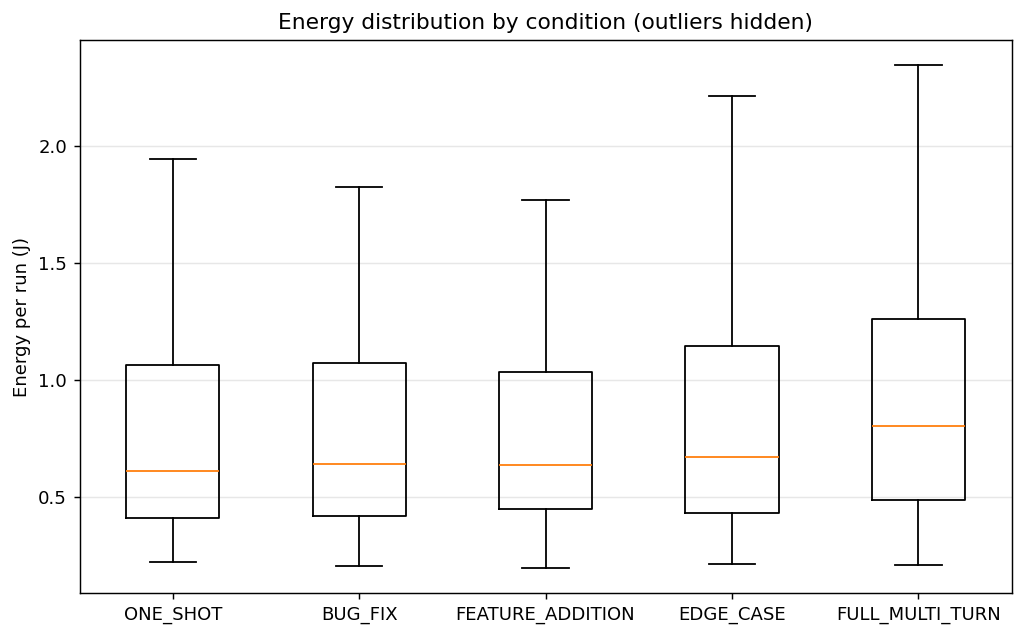
\includegraphics[width=\columnwidth]{images/fig01_energy_box.png}
\caption{Energy distribution by interaction condition. Multi-turn shifts the
median up and thickens the upper tail (heavy-tail effect).}
\label{fig:box}
\end{figure}

\begin{figure}[htbp]
\centering
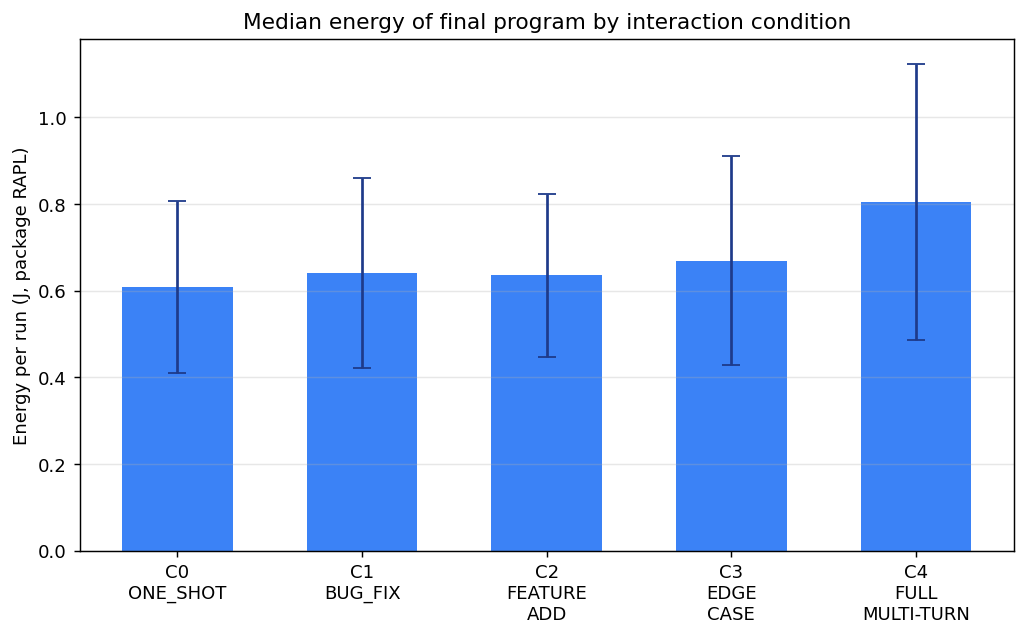
\includegraphics[width=\columnwidth]{images/fig02_median_energy.png}
\caption{Median energy by condition. The C0$\rightarrow$C4 step (+32\%) is
the largest single increase.}
\label{fig:med}
\end{figure}

\subsection{Paired analysis: \texorpdfstring{$\Delta E$}{dE} versus one-shot (RQ1, RQ3)}\index{paired analysis}
Within-(task, model) pairing (Table~\ref{tab:paired},
Figs.~\ref{fig:delta}--\ref{fig:scatter}) shows only the full multi-turn
trajectory reaching significance ($p{=}0.006$): the cumulative trajectory,
not any single step, drives the increase. Bug-fix is a wash (median
$-0.4$\%, wins/losses 131/132); feature (+2.3\%) and edge-case (+2.5\%) are
positive but insignificant; the full trajectory compounds to mean +232.1\%
and median +3.7\%.

\begin{table}[htbp]
\caption{Paired energy change vs.\ one-shot within (task, model). Only C4 is
significant (Wilcoxon $p{=}0.006$).}
\label{tab:paired}
\centering
\begin{tabular}{lcccccc}
\toprule
Cond. & $n$ & Mean\% & Med.\% & $\uparrow$ & $\downarrow$ & $p$ \\
\midrule
C1 & 263 & +25.9 & $-0.4$ & 131 & 132 & 0.869 \\
C2 & 253 & +81.2 & +2.3 & 141 & 112 & 0.122 \\
C3 & 249 & +137.8 & +2.5 & 135 & 114 & 0.251 \\
C4 & 224 & +232.1 & +3.7 & 127 & 97 & 0.006 \\
\bottomrule
\end{tabular}
\end{table}

\begin{figure}[htbp]
\centering
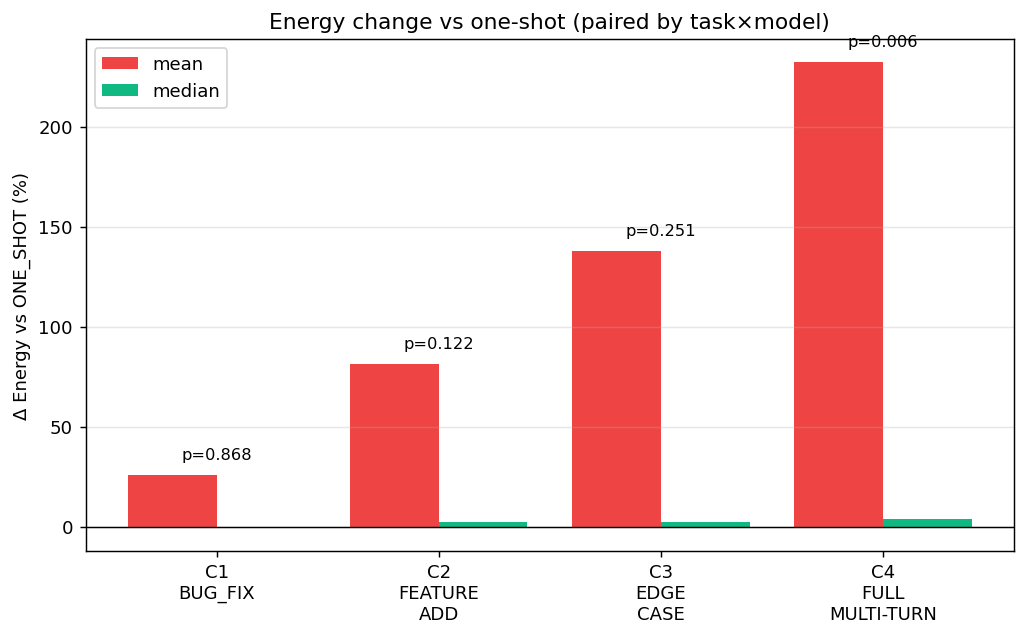
\includegraphics[width=\columnwidth]{images/fig03_paired_delta.png}
\caption{Paired per-program energy change ($\Delta E$ \%) vs.\ one-shot, by
condition. Only C4 separates from zero significantly.}
\label{fig:delta}
\end{figure}

\begin{figure}[htbp]
\centering
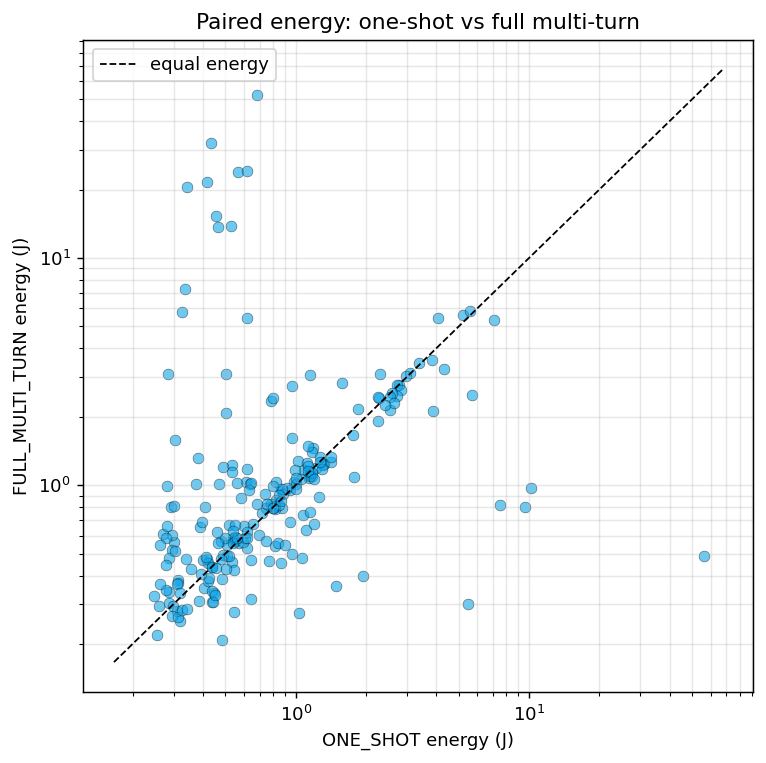
\includegraphics[width=\columnwidth]{images/fig04_oneshot_vs_multiturn.png}
\caption{Paired scatter: one-shot vs.\ full multi-turn energy per
(task, model). Points above the diagonal cost more after the trajectory.}
\label{fig:scatter}
\end{figure}

\subsection{Effect of individual interaction steps (RQ3)}
No single step moves the median more than a few percent, yet each step
raises the \emph{mean} substantially (+26\% bug-fix, +81\% feature, +138\%
edge-case). The pattern---stable medians, inflating means---indicates each
turn adds a chance of a large regression rather than a uniform tax, with the
full trajectory compounding independent per-turn risks.

\subsection{Model-specific effects (RQ2)}
The uplift direction is consistent across all four models but absolute
levels and magnitudes differ sharply (Table~\ref{tab:bymodel},
Fig.~\ref{fig:bymodel}). Claude writes the longest, most branched code
(median SLOC 93, cyclomatic 18) and shows the highest median energy
(0.874\,J) and largest mean uplift (+557\%); Gemini is the leanest (SLOC 61,
cyclomatic 13, 0.565\,J). GPT and DeepSeek fall between. The model ranking
in energy mirrors the model ranking in code size and branching, foreshadowing
Section~\ref{sec:results-mediation}.

\begin{table}[htbp]
\caption{Mean energy (J) by condition and model; right column is mean paired
uplift vs.\ one-shot.}
\label{tab:bymodel}
\centering
\begin{tabular}{lccccc|c}
\toprule
Model & C0 & C1 & C2 & C3 & C4 & Mean $\Delta$ \% \\
\midrule
GPT & 1.550 & 0.823 & 0.825 & 0.787 & 1.305 & +90.6 \\
Claude & 0.967 & 1.054 & 1.491 & 2.054 & 3.387 & +556.6 \\
Gemini & 1.196 & 1.603 & 1.084 & 1.148 & 2.029 & +146.9 \\
DeepSeek & 1.206 & 0.953 & 1.605 & 2.134 & 1.423 & +161.6 \\
\bottomrule
\end{tabular}
\end{table}

\begin{figure}[htbp]
\centering
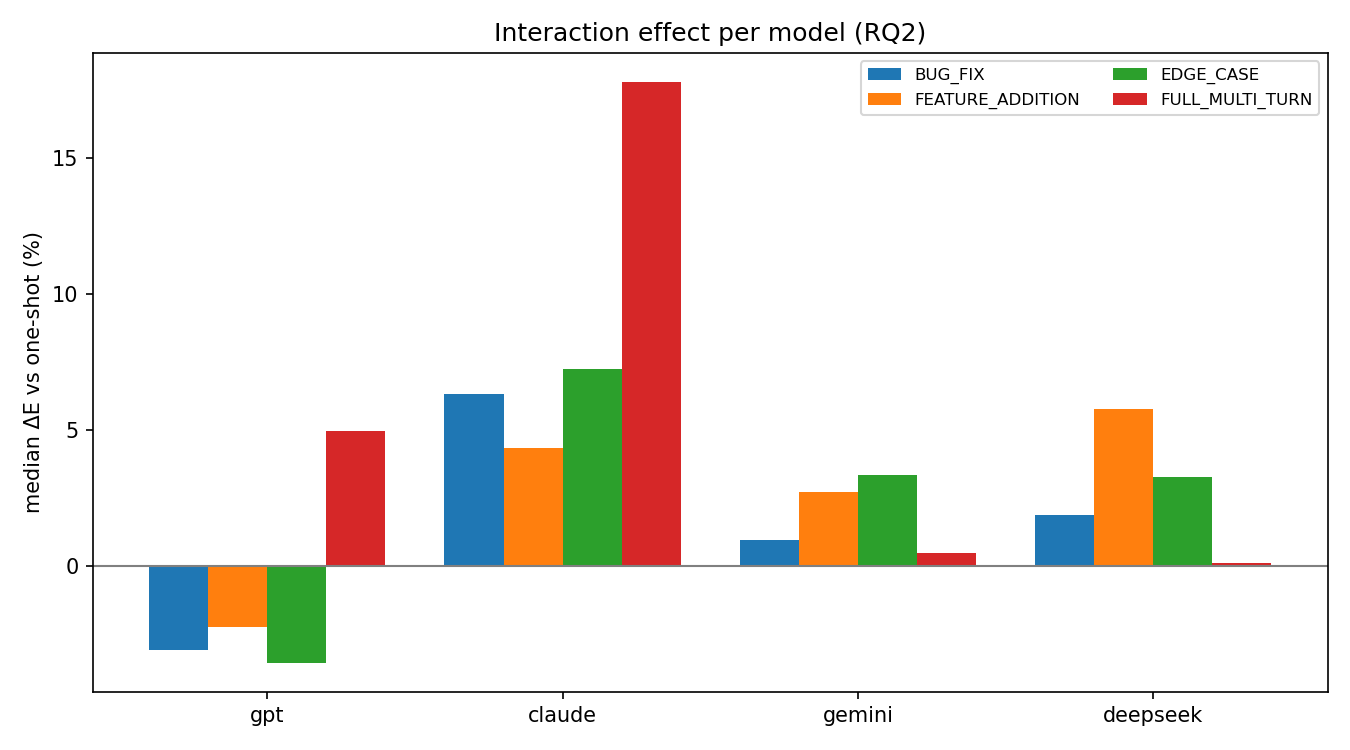
\includegraphics[width=\columnwidth]{images/fig05_energy_by_model.png}
\caption{Energy by condition, faceted by model. Direction is consistent;
magnitude varies by vendor.}
\label{fig:bymodel}
\end{figure}

\begin{table}[htbp]
\caption{Model code style vs.\ energy (condition-pooled medians). Verbose,
branchy models cost more to run.}
\label{tab:modelstyle}
\centering
\begin{tabular}{lcccc}
\toprule
Model & Med.\ SLOC & Med.\ cyclo. & Med.\,J & \% quadr.+ \\
\midrule
Claude & 93.0 & 18 & 0.874 & 52.7 \\
DeepSeek & 83.0 & 18 & 0.672 & 53.6 \\
GPT & 58.5 & 11 & 0.604 & 43.7 \\
Gemini & 61.0 & 13 & 0.567 & 44.3 \\
\bottomrule
\end{tabular}
\end{table}

\subsection{Category-specific effects}
Algorithms tasks show the largest mean uplift (+732\%)---unsurprising, since
only there can a trajectory substitute an asymptotically worse algorithm for
a better one (Table~\ref{tab:bycat}, Fig.~\ref{fig:bycat}). Image/media
workloads, dominated by fixed-cost library calls, move least (+12.8\%).
Absolute levels invert the pattern: media programs are the most expensive
per run (median 1.147\,J) and text/log the cheapest (0.416\,J), reflecting
workload weight rather than trajectory sensitivity
(Table~\ref{tab:bycatabs}).

\begin{table}[htbp]
\caption{Energy change by category (mean paired uplift vs.\ one-shot).}
\label{tab:bycat}
\centering
\begin{tabular}{lcc}
\toprule
Category & Units & Mean $\Delta E$ \% \\
\midrule
Algorithms \& Comp. & 407 & +732.5 \\
File \& Data & 326 & +34.2 \\
Image \& Media & 367 & +12.8 \\
Realistic Apps & 113 & +278.6 \\
Text \& Log & 94 & +110.1 \\
\bottomrule
\end{tabular}
\end{table}

\begin{figure}[htbp]
\centering
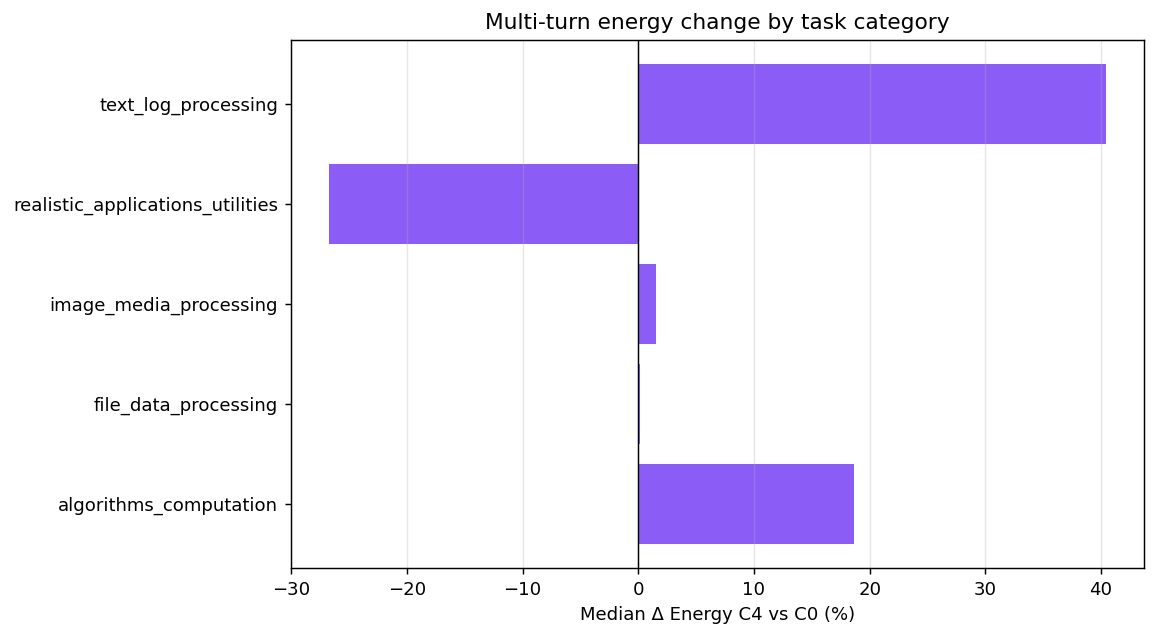
\includegraphics[width=\columnwidth]{images/fig12_delta_by_category.png}
\caption{Mean energy change vs.\ one-shot by task category. Algorithmic
tasks dominate the uplift.}
\label{fig:bycat}
\end{figure}

\begin{table}[htbp]
\caption{Absolute levels by category (condition-pooled medians). Heavy
fixed-cost workloads (media) cost most per run regardless of trajectory.}
\label{tab:bycatabs}
\centering
\begin{tabular}{lccc}
\toprule
Category & Med.\,J & Med.\ SLOC & \% quadr.+ \\
\midrule
Algorithms \& Comp. & 0.494 & 87.0 & 85.5 \\
File \& Data & 0.803 & 80.0 & 44.2 \\
Image \& Media & 1.147 & 52.0 & 25.9 \\
Realistic Apps & 0.545 & 91.0 & 23.0 \\
Text \& Log & 0.416 & 60.0 & 22.3 \\
\bottomrule
\end{tabular}
\end{table}

\subsection{Runtime, power, and memory (RQ4)}
Runtime and energy are almost collinear (Spearman $\rho{=}0.9328$, Pearson
$r{=}0.9952$, $n{=}1307$): package energy in this workload is
runtime-dominated (Fig.~\ref{fig:rte}). Average power is strikingly flat
across conditions (8.61--8.80\,W medians, Table~\ref{tab:powermem})---the
trajectory effect operates through \emph{time}, not wattage. Peak memory
rises modestly (11.65\,MB $\rightarrow$ 13.54\,MB medians; paired mean
+1.32\,MB), consistent with accumulated state and buffering across turns.

\begin{figure}[htbp]
\centering
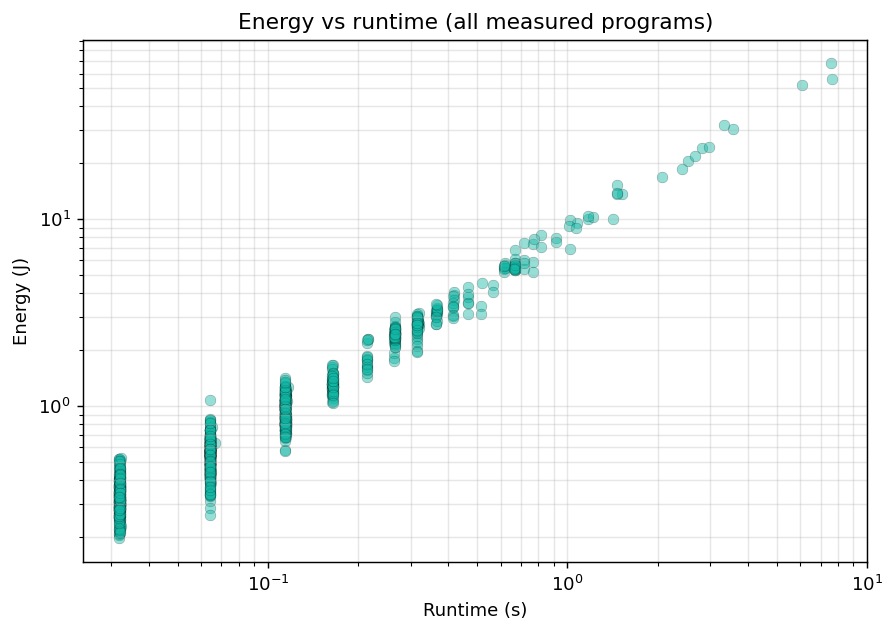
\includegraphics[width=\columnwidth]{images/fig06_runtime_vs_energy.png}
\caption{Runtime vs.\ package energy (log--log). Energy is
runtime-dominated; the C4 cloud extends to longer runtimes.}
\label{fig:rte}
\end{figure}

\begin{table}[htbp]
\caption{Power, memory, and runtime medians by condition. Power is flat;
time and memory grow with trajectory length.}
\label{tab:powermem}
\centering
\begin{tabular}{lcccc}
\toprule
Cond. & Power (W) & Peak mem (MB) & Runtime (s) & SLOC \\
\midrule
C0 & 8.75 & 11.65 & 0.0641 & 56.0 \\
C1 & 8.61 & 11.49 & 0.0642 & 61.5 \\
C2 & 8.80 & 12.23 & 0.0642 & 79.0 \\
C3 & 8.75 & 12.49 & 0.0642 & 77.0 \\
C4 & 8.71 & 13.54 & 0.1142 & 94.0 \\
\bottomrule
\end{tabular}
\end{table}

\subsection{Static code metrics (RQ5)}
Size and structural complexity grow monotonically C0$\rightarrow$C4
(Table~\ref{tab:static}, Fig.~\ref{fig:sloc}). The paired view
(Table~\ref{tab:pairstatic}) is sharper: the full trajectory adds on average
58 lines (median +35; 81.6\% of programs grow), +9.0 cyclomatic points
(median +5), and +1.9 functions---while loop depth and complexity rank are
unchanged on average. Trajectories inflate programs without deepening loop
nests: breadth, not depth.

\begin{table}[htbp]
\caption{Static metrics by condition (medians).}
\label{tab:static}
\centering
\begin{tabular}{lccccc}
\toprule
Cond. & SLOC & Func. & Cyclo. & Rank & \%Q+ \\
\midrule
C0 & 56.0 & 2 & 13 & 1.5 & 48.6 \\
C1 & 61.5 & 2 & 14 & 1.5 & 49.6 \\
C2 & 79.0 & 2 & 14 & 1.5 & 49.8 \\
C3 & 77.0 & 2 & 15.5 & 1.5 & 47.7 \\
C4 & 94.0 & 3 & 18 & 1.5 & 46.6 \\
\bottomrule
\end{tabular}
\end{table}

\begin{figure}[htbp]
\centering
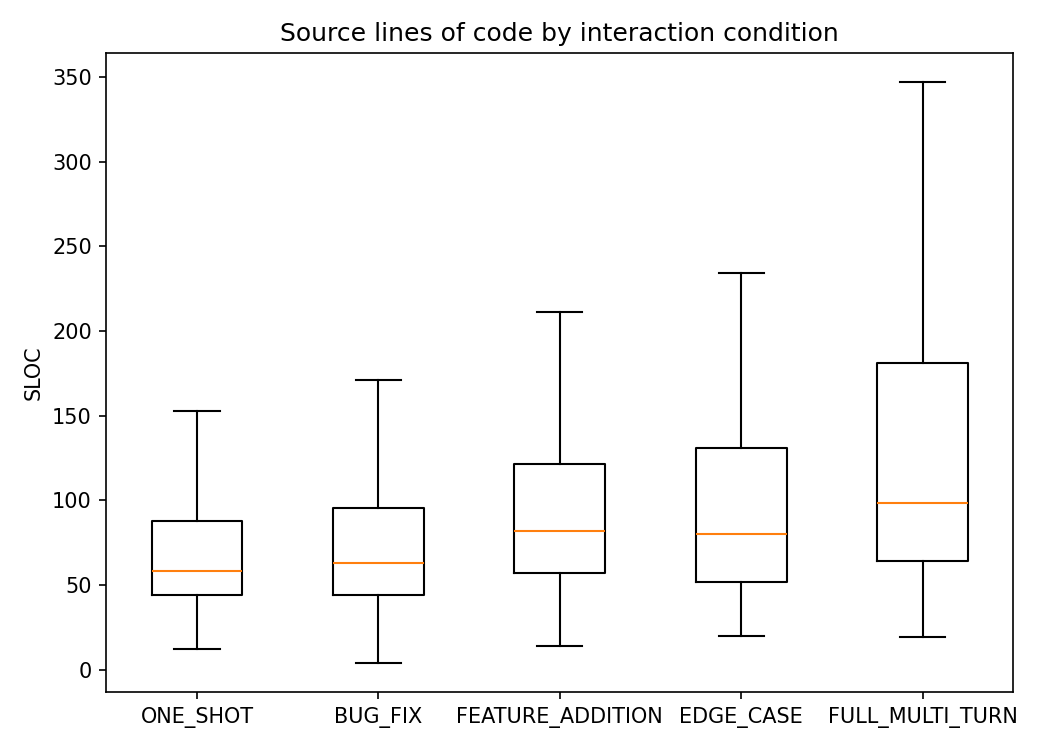
\includegraphics[width=\columnwidth]{images/fig07_sloc_by_condition.png}
\caption{SLOC distribution by condition (median 94 vs.\ 56 for C4
vs.\ C0).}
\label{fig:sloc}
\end{figure}

\begin{table}[htbp]
\caption{Paired static deltas C4 vs.\ C0 within (task, model). Trajectories
add breadth (lines, branches, functions), not depth.}
\label{tab:pairstatic}
\centering
\begin{tabular}{lcccc}
\toprule
Metric & $n$ & Mean $\Delta$ & Med.\ $\Delta$ & \% growing \\
\midrule
SLOC & 272 & +58.3 & +34.5 & 81.6 \\
Cyclomatic & 272 & +9.0 & +5.0 & 76.1 \\
Functions & 272 & +1.9 & +1.0 & 52.2 \\
Complexity rank & 272 & +0.03 & 0.0 & 16.2 \\
Max loop depth & 272 & $-0.01$ & 0.0 & 8.8 \\
\bottomrule
\end{tabular}
\end{table}

\subsection{Time-complexity distribution (RQ5)}
The estimated-class mix is dominated by linear and linearithmic programs
with a substantial quadratic-plus tail
(Table~\ref{tab:dist}, Fig.~\ref{fig:mix}). Notably, the quadratic-plus
share is essentially flat across conditions (46.6--49.8\%): trajectories add
code without shifting the \emph{class} mix---regressions hide inside classes
(e.g.\ larger constants, extra passes) or in the small superlinear tail.

\begin{table}[htbp]
\caption{Estimated time-complexity class distribution ($n{=}1418$).}
\label{tab:dist}
\centering
\begin{tabular}{lc}
\toprule
Estimated class & Programs \\
\midrule
$O(n\log n)$ & 379 \\
$O(n)$ & 295 \\
$O(n^2\log n)$ & 276 \\
$O(n^2)$ & 258 \\
$O(n^3)$ & 93 \\
$O(2^n)$ & 50 \\
$O(n^4)$ & 43 \\
$O(1)$ & 24 \\
\bottomrule
\end{tabular}
\end{table}

\begin{figure}[htbp]
\centering
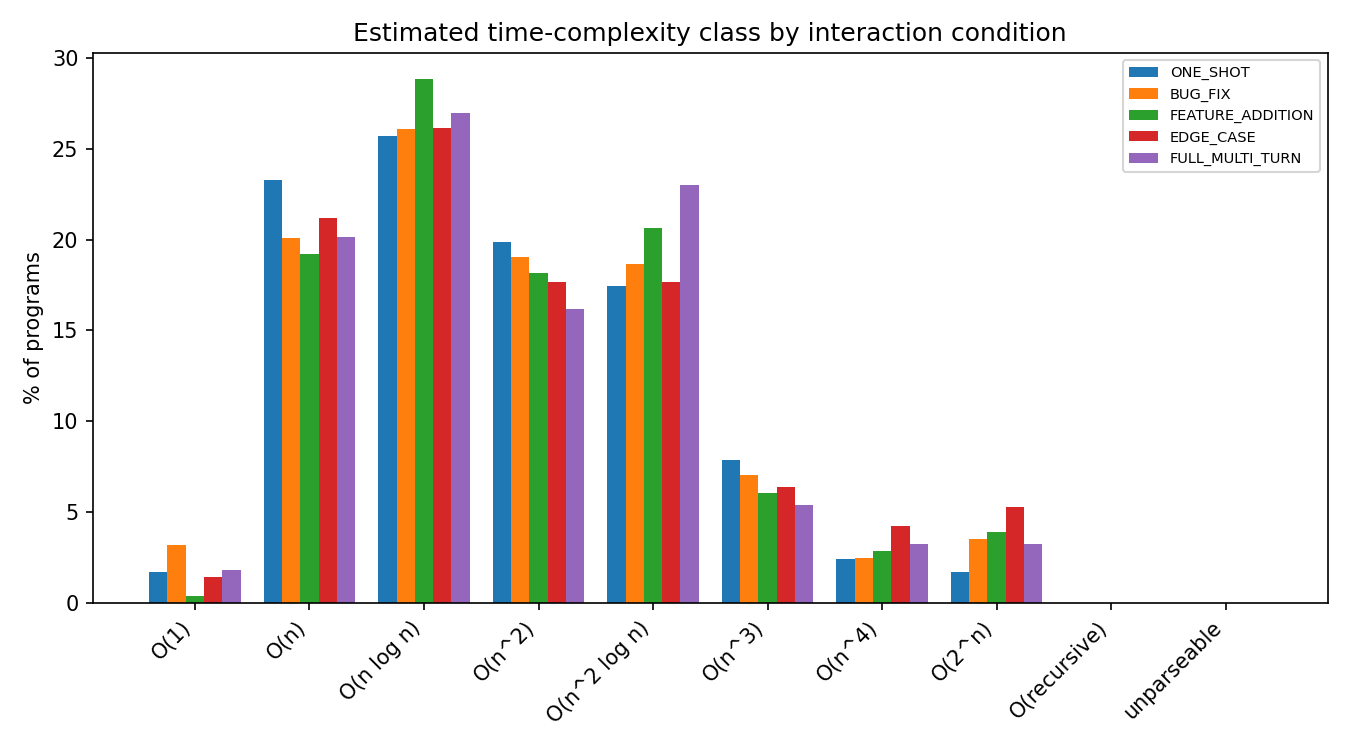
\includegraphics[width=\columnwidth]{images/fig08_complexity_mix.png}
\caption{Estimated complexity-class mix by condition. The quadratic-plus
share is stable; C4 adds SLOC within classes.}
\label{fig:mix}
\end{figure}

\subsection{Estimated versus empirical complexity}\label{sec:results-complex}
Across 59 programs with both estimates, Spearman(rank,
slope)$\,{=}\,{-}0.114$. As a binary superlinear classifier (rank $\geq$2
vs.\ slope $\geq$1.5): precision 0.226, recall 0.875 (TP=7, FP=24, FN=1,
TN=27, Table~\ref{tab:agree}). High recall with low precision is the
expected trade-off for a conservative AST rule: it rarely misses true
superlinear behaviour but over-flags it. Reliable-slope medians (candidate
1.02 vs.\ reference 1.12) confirm the harness scales near-linearly and the
probe is calibrated (Fig.~\ref{fig:slope}).

\begin{table}[htbp]
\caption{Agreement: static estimator vs.\ empirical slope ($n{=}59$;
precision 0.226, recall 0.875).}
\label{tab:agree}
\centering
\begin{tabular}{lcc}
\toprule
 & Slope $<1.5$ & Slope $\geq1.5$ \\
\midrule
Rank $<2$ & 27 & 1 \\
Rank $\geq2$ & 24 & 7 \\
\bottomrule
\end{tabular}
\end{table}

\begin{figure}[htbp]
\centering
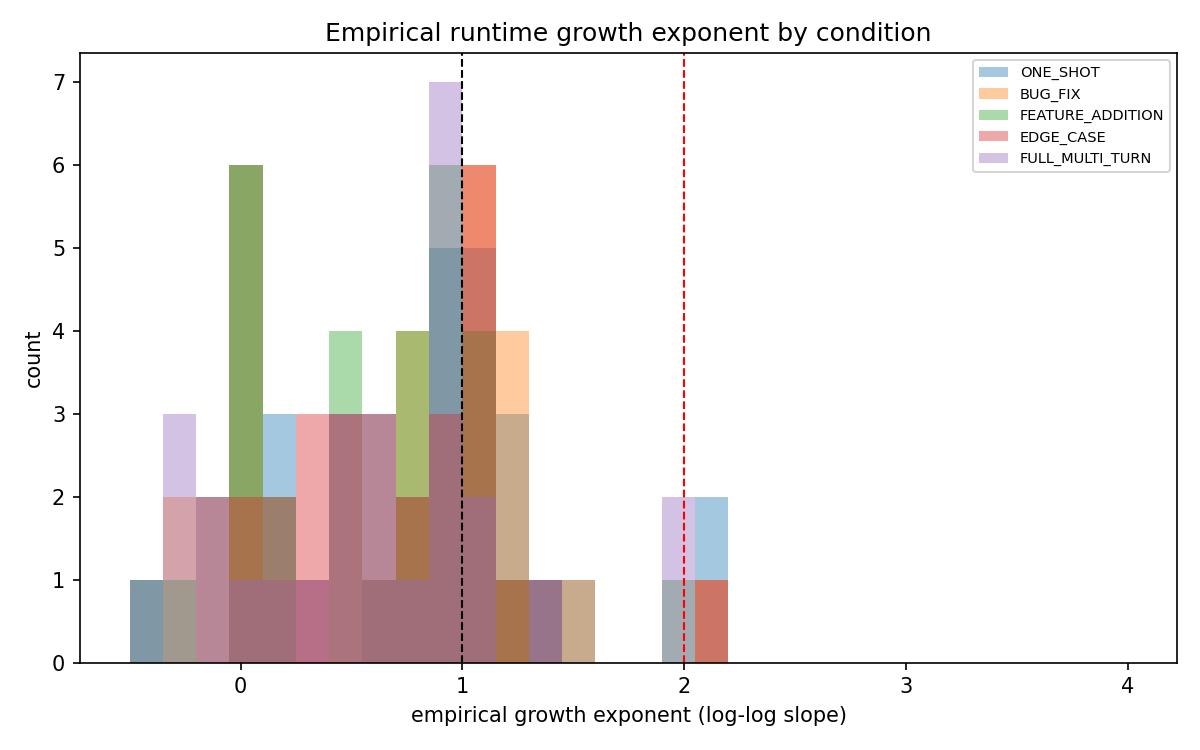
\includegraphics[width=\columnwidth]{images/fig09_slope_hist.png}
\caption{Empirical growth-exponent distribution. Most programs scale
near-linearly; the superlinear tail is small but real.}
\label{fig:slope}
\end{figure}

\subsection{Complexity, size, and energy: mediation (RQ5)}\label{sec:results-mediation}
Code-level complexity correlates weakly with energy across heterogeneous
tasks (SLOC--energy $\rho{=}0.04$; rank--energy $\rho{=}{-}0.15$; loop
depth--energy $\rho{=}{-}0.29$), whereas runtime correlates almost perfectly
($\rho{=}0.93$, Table~\ref{tab:corr}). The multi-turn energy penalty is
therefore transmitted through longer or heavier \emph{executions}, not
through source-level complexity per se---a mediation pattern with direct
tooling consequences (Section~\ref{sec:discuss-tools}): monitor scaling
behaviour, not line counts.

\begin{table}[htbp]
\caption{Cross-metric correlations on measured programs ($n{=}1307$).}
\label{tab:corr}
\centering
\begin{tabular}{lcc}
\toprule
Pair & Spearman $\rho$ & Pearson $r$ \\
\midrule
Runtime vs.\ energy & 0.9328 & 0.9952 \\
SLOC vs.\ runtime & 0.0070 & 0.0756 \\
SLOC vs.\ energy & 0.0389 & 0.0755 \\
Cyclomatic vs.\ energy & $-0.0758$ & 0.0570 \\
Complexity rank vs.\ energy & $-0.1529$ & 0.0405 \\
Loop depth vs.\ energy & $-0.2862$ & $-0.0371$ \\
\bottomrule
\end{tabular}
\end{table}

\subsection{Carbon-equivalent emissions (RQ6)}\label{sec:results-carbon}
The 1307 measured programs consumed 1852.1\,J $=$ 246.9\,mgCO$_{2}$eq at the
global-average intensity (Table~\ref{tab:carbon}, Fig.~\ref{fig:carbon}).
Condition rankings are intensity-invariant: the median multi-turn run costs
107.3\,$\upmu$g vs.\ 81.2\,$\upmu$g one-shot (+26.1\,$\upmu$g), and the mean
overhead is $\approx$106\,$\upmu$g/run (0.792\,J $\times$ 480\,g/kWh).
Section~\ref{sec:discuss-carbon} scales these unit economics to deployment.

\begin{table}[htbp]
\caption{Carbon sensitivity by grid intensity (medians per run; total for
the measured corpus).}
\label{tab:carbon}
\centering
\begin{tabular}{lcccc}
\toprule
Grid & g/kWh & C0 $\upmu$g & C4 $\upmu$g & Total mg \\
\midrule
Global average & 480 & 81.2 & 107.3 & 246.9 \\
US average & 369 & 62.4 & 82.5 & 189.8 \\
EU average & 251 & 42.5 & 56.1 & 129.1 \\
Low-carbon & 56 & 9.5 & 12.5 & 28.8 \\
\bottomrule
\end{tabular}
\end{table}

\begin{figure}[htbp]
\centering
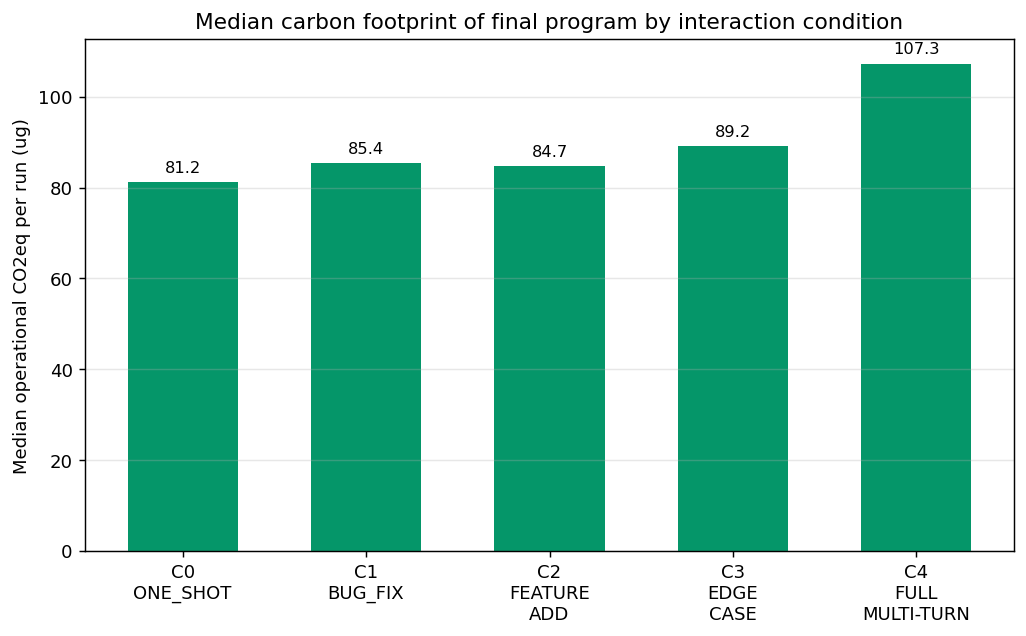
\includegraphics[width=\columnwidth]{images/fig10_carbon.png}
\caption{Carbon-equivalent by condition across grid intensities. Rankings
are intensity-invariant; geography scales totals $\approx$9$\times$.}
\label{fig:carbon}
\end{figure}

\subsection{Failure taxonomy and coverage bias}\label{sec:results-fail}\index{failure taxonomy}
111 units carry genuine model-output failures, led by
\texttt{WRONG\_OUTPUT} (78)---embedded self-test failures (logic bugs in
generated code)---then runtime bugs (33). A further 65 unmeasured units are
collection artifacts, excluded from every analysis: prose submitted instead
of code (14), harness-invocation mismatches (43 across \texttt{CLI\_ARGS},
\texttt{OTHER}, and \texttt{SILENT\_RC1}), programs assuming inputs the
harness never provided (3), and modules missing from the sandbox (5).
Failures concentrate in algorithms (82 of 111 genuine failures). Coverage is
thus biased toward harness-clean programs; paired
tests (units present in both conditions) bound this bias, and the
monotone failure gradient itself (Table~\ref{tab:failrate},
Fig.~\ref{fig:fail}) is a finding: interaction depth degrades executability.

\begin{figure}[htbp]
\centering
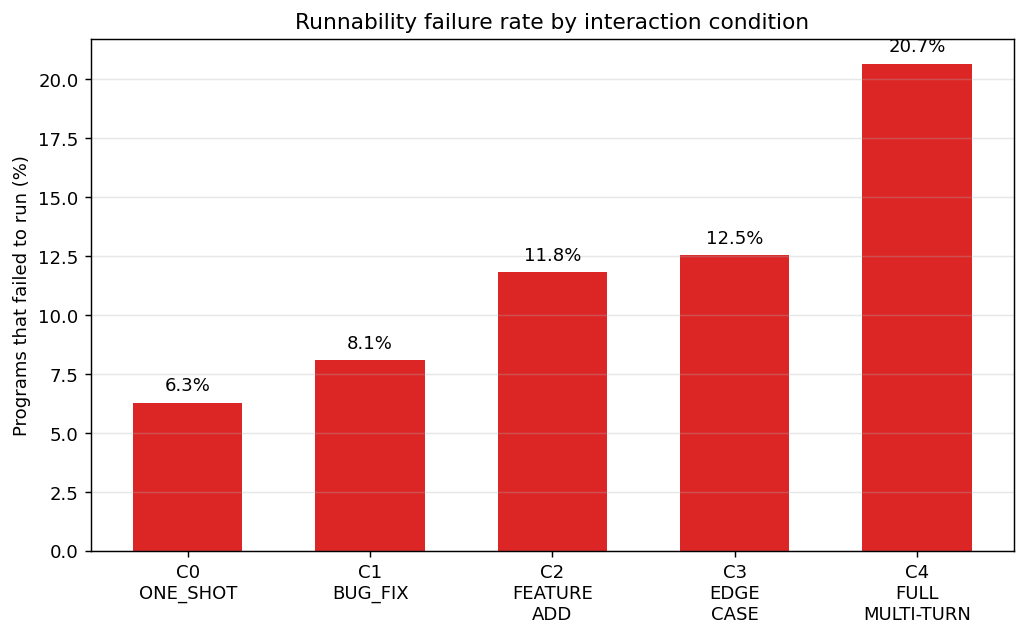
\includegraphics[width=\columnwidth]{images/fig11_failure_rate.png}
\caption{Genuine model-failure rate by condition (collection artifacts
excluded). Full multi-turn fails most
often---complexity has a correctness cost too.}
\label{fig:fail}
\end{figure}

\section{Discussion}\label{sec:discussion}
\subsection{Interpretation of main findings}
Multi-turn interaction leaves a measurable green-software footprint with a
distinctive signature: stable medians for single steps, an inflating mean at
every step, and significance only for the full trajectory. Practically, most
sessions cost little extra while a minority cost a great deal---the classic
heavy tail that means-based capacity planning must respect and median-based
reporting would hide.

\subsection{Why multi-turn programs consume more energy}
Three compounding mechanisms, each grounded in the measurements: (i)
\emph{accumulation}---requirements pile up into longer, less pruned code
(+58 mean SLOC; 82\% of programs grow); (ii) \emph{defensiveness}---feature
and edge turns add branches and extra input passes (cyclomatic 13
$\rightarrow$ 18; paired +9.0); (iii) \emph{asymptotic drift}---some
trajectories settle on heavier algorithms, visible as superlinear empirical
slopes (C4 reliable-slope superlinear rate 18\% vs.\ 6\% overall) and the
enormous algorithms-category mean uplift (+732\%).

\subsection{Complexity as a mediator}
Static complexity rises with depth yet correlates weakly with energy; the
mediator is runtime. This resolves an apparent paradox in
Table~\ref{tab:static} (flat class mix) versus Table~\ref{tab:energy}
(rising energy): regressions occur \emph{within} complexity classes. The
leverage point for intervention is therefore algorithmic-scaling behaviour,
not line counts---a conclusion that favours dynamic profiling and scaling
tests over SLOC budgets.

\subsection{Carbon and environmental implications (RQ6)}\label{sec:discuss-carbon}\index{carbon effect}
Measured unit economics first: at the global-average grid, the median
multi-turn run carries +26.1\,$\upmu$gCO$_{2}$eq over one-shot and the mean
+106\,$\upmu$g. These are negligible per run by construction---a single
program execution is cheap. Scale changes the picture (illustrative
projections, not measurements): one million multi-turn executions add
$\approx$26\,g (median) to $\approx$106\,g (mean) CO$_{2}$eq; one hundred
million add $\approx$2.6--10.6\,kg; a platform serving ten million assisted
sessions daily accrues $\approx$0.26--1.06\,kg/day from this overhead alone,
before counting inference energy, which dominates today. Geography matters
as much as volume: moving execution from an average to a low-carbon grid
cuts totals $\approx$9$\times$ (247\,mg $\rightarrow$ 29\,mg for our
corpus), a larger lever than any trajectory optimisation we observe.
To put a single run in perspective: the median multi-turn execution
($\approx$107\,$\upmu$gCO$_{2}$eq) is roughly one thirty-five-thousandth of
a smartphone charge ($\approx$3.8\,gCO$_{2}$eq)---the environmental question
is never one program but the aggregate of billions of executions. At one
billion executions the mean multi-turn overhead alone ($\approx$107\,kg)
is comparable to $\approx$620\,km of average car driving or the CO$_{2}$
sequestered by $\approx$5 tree-years.

\emph{Scope of the estimate.} This is \emph{operational} carbon from
\emph{CPU package energy only}; it excludes DRAM/GPU energy, platform idle
power, embodied carbon, and---crucially---the energy of LLM inference
during code generation, which dominates the total human--AI coding cost. It
is therefore a lower bound on runtime emissions and a statement about the
\emph{runtime footprint of the final program}, not the end-to-end footprint
of the interaction.

Four effects make real-world impact larger than raw $\Delta E$ suggests:
(1)~\emph{participation multiplier}---with tens of millions of developers,
ratios survive aggregation; (2)~\emph{rework waste}---multi-turn finals fail
$\approx$5$\times$ more often (15.8\% vs.\ 3.4\%), and each failed run still
burns CPU while retries add unmeasured energy, so our successful-run
comparison under-counts the penalty; (3)~\emph{tail blow-ups}---the worst
program in the corpus (AC-012, deepseek edge-case, 67.9\,J) emits
$\approx$9.1\,mgCO$_{2}$eq per run, $\approx$85$\times$ the median, and if
such patterns recur across a fleet the tail drives totals; (4)~\emph{rebound
(Jevons) effects}---cheaper generation increases total software volume.
Countervailing evidence keeps the story honest: the bug-fix turn alone moves
median energy by $-0.1$\%, so not all iteration is harmful---\emph{how} the
trajectory is used determines the sign, not whether AI is used.

Two caveats keep this honest. First, operational overhead must be weighed
against \emph{avoided} costs: if iteration produces correct code faster,
fewer human-machine hours and fewer broken deployments may offset the
per-run penalty---a full lifecycle comparison is future work. Second,
efficiency gains invite rebound: cheaper iteration encourages more
iteration. The policy-relevant reading is therefore not ``never iterate''
but ``make iteration costs visible and prune by default'': complexity
reviews at session end, scaling smoke-tests in CI for generated code, and
carbon-aware scheduling of heavy generated workloads.

\subsection{Implications for practitioners}
Treat iterative features as potential complexity regressions and re-benchmark
the final artifact, not just the first draft. Ask assistants to justify
asymptotic cost after each turn, not only at the end. Close lengthening
sessions with a pruning pass: our paired data show 4 of 5 programs grow and
only half gain functions, i.e.\ much added code is bulk, not structure.

\subsection{Implications for tool builders}\label{sec:discuss-tools}
IDE-integrated green linters should surface per-turn estimated complexity
and measured energy deltas---e.g.\ flagging a turn that moves the estimate
from $O(n\log n)$ to $O(n^2)$, or a session whose runtime doubled since the
first draft. Because the penalty is heavy-tailed, tools should alert on
outliers (large $\Delta E$) rather than taxing every turn. Session-level
``energy receipts'' (total joules across drafts, not just the final) would
extend this benchmark's final-artifact view to full lifecycle accounting.

\subsection{Research agenda}
We see five directions: (1)~per-turn energy attribution across entire
sessions, including inference cost; (2)~automatic complexity-regression
detection during interactive coding; (3)~lifecycle studies weighing
operational overhead against avoided developer and deployment costs;
(4)~replication across languages, hardware (including non-RAPL power
measurement), and model families; (5)~full-category empirical scaling sweeps
with finer input-size grids.

\section{Threats to Validity}\label{sec:threats}\index{threats to validity}
\emph{Construct validity.} RAPL package energy includes off-target
components; identical workloads, warm-up, repetition, and paired
within-(task, model) differencing mitigate but do not eliminate noise. The
static Big-O estimator is an explicit heuristic---its limits are quantified
(precision 0.226) rather than hidden, and it is cross-checked against both
declared targets and measured slopes.

\emph{Internal validity.} Deterministic shared workloads and paired tests
control task difficulty. The 111 genuine model failures bias coverage toward
runnable programs; the monotone failure gradient (3.4\% $\rightarrow$ 15.8\%)
means C4-vs-C0 comparisons condition on survivorship, likely
\emph{understating} the true trajectory cost since the worst C4 programs
never ran. The 65 excluded collection artifacts are documented in
Section~\ref{sec:results-fail}, not silently dropped.

\emph{External validity.} One host microarchitecture, Python only, four
model families, one time window. Absolute joules will differ elsewhere; the trajectory \emph{pattern}
(median-stable steps, significant full trajectory, heavy tail) is the
portable claim and needs replication.

\emph{Conclusion validity.} Only C4 reaches significance---single-step
claims are withheld despite suggestive means. The empirical probe covers the
algorithms category; static metrics cover all 1418. Reliable-slope
filtering ($\geq$5\,ms) excludes overhead-dominated fits; unfiltered results
are available in the corpus for re-analysis.

\section{Conclusion and Future Work}\label{sec:conclusion}
Holding the final specification constant, full multi-turn AI-assisted
trajectories increase the median package energy of generated programs by
one-third and the mean by two-thirds relative to one-shot generation---the
only statistically significant effect---mediated by runtime and algorithm
choice rather than source size, and accompanied by higher failure rates. We
release a per-program corpus (energy, runtime, memory, power, static
metrics, dual complexity estimates, carbon translations) with full
reproduction scripts. The practical takeaway is targeted, not prohibitive:
iterate, but instrument each turn, review complexity at session end, and
schedule heavy generated workloads on low-carbon capacity.

\section*{Author Contributions}
All authors contributed equally to task design, interaction design,
measurement, analysis, and writing.

\section*{Acknowledgment}
We thank the compute and measurement host providers and the maintainers of
Intel RAPL tooling, Python, and the open model ecosystem. [Funding/grant
acknowledgments to be added.]

\begin{thebibliography}{00}
\bibitem{rotem2012} E.~Rotem et al., ``Power-management architecture of the
Intel microarchitecture code-named Sandy Bridge,'' \emph{IEEE Micro},
vol.~32, no.~2, pp.~20--27, 2012.
\bibitem{david2010} H.~David et al., ``RAPL: Memory power estimation and
capping,'' in \emph{Proc.\ ISLPED}, 2010.
\bibitem{hahnell2012} M.~H\"ahn et al., ``Measuring energy consumption for
short code paths using RAPL,'' \emph{ACM SIGMETRICS PER}, vol.~40, no.~3,
pp.~13--17, 2012.
\bibitem{hackenberg2013} D.~Hackenberg et al., ``An energy efficiency feature
survey of the Intel Haswell processor,'' in \emph{Proc.\ IPDPSW}, 2013.
\bibitem{schwartz2020} R.~Schwartz et al., ``Green AI,'' \emph{Commun.\ ACM},
vol.~63, no.~12, pp.~54--63, 2020.
\bibitem{strubell2019} E.~Strubell et al., ``Energy and policy considerations
for deep learning in NLP,'' in \emph{Proc.\ ACL}, 2019.
\bibitem{patterson2021} D.~Patterson et al., ``Carbon emissions and large
neural network training,'' arXiv:2104.10350, 2021.
\bibitem{luccioni2022} A.~S.~Luccioni et al., ``Estimating the carbon
footprint of BLOOM, a 176B parameter language model,'' \emph{J.\ Mach.\
Learn.\ Res.}, vol.~24, pp.~1--15, 2023.
\bibitem{lacoste2019} A.~Lacoste et al., ``Quantifying the carbon emissions
of machine learning,'' arXiv:1910.09700, 2019.
\bibitem{henderson2020} P.~Henderson et al., ``Towards the systematic
reporting of the energy and carbon footprints of machine learning,''
\emph{J.\ Mach.\ Learn.\ Res.}, vol.~21, pp.~1--43, 2020.
\bibitem{codecarbon2021} J.~Schmidt et al., ``CodeCarbon: Estimate and track
carbon emissions from ML computing,'' GitHub, 2021.
\bibitem{verdecchia2023} R.~Verdecchia et al., ``A systematic review of green
AI,'' \emph{WIREs Data Mining Knowl.\ Discov.}, vol.~13, no.~4, 2023.
\bibitem{pereira2017} R.~Pereira et al., ``Energy efficiency across
programming languages,'' in \emph{Proc.\ SLE}, 2017.
\bibitem{pinto2014} G.~Pinto et al., ``Understanding energy behaviors of
thread management constructs,'' in \emph{Proc.\ OOPSLA}, 2014.
\bibitem{pinto2014b} G.~Pinto et al., ``Energy efficiency: A new concern for
software engineers,'' in \emph{Proc.\ SAC}, 2014.
\bibitem{georgiou2022} S.~Georgiou et al., ``Green AI: Do deep learning
frameworks have different costs?'' \emph{Empir.\ Softw.\ Eng.}, vol.~27,
2022.
\bibitem{calero2015} C.~Calero and M.~Piattini, Eds., \emph{Green in Software
Engineering}, Springer, 2015.
\bibitem{hindle2023} A.~Hindle, ``Green software engineering: The curse of
methodology,'' \emph{Empir.\ Softw.\ Eng.}, 2023.
\bibitem{hotcarbon2022} A.~Anwar et al., ``Datacenter-scale energy and carbon
accounting,'' in \emph{Proc.\ HotCarbon}, 2022.
\bibitem{spec2008} Standard Performance Evaluation Corporation,
``SPECpower\_ssj2008,'' 2008.
\bibitem{chen2021} M.~Chen et al., ``Evaluating large language models trained
on code,'' arXiv:2107.03374, 2021.
\bibitem{austin2021} J.~Austin et al., ``Program synthesis with large language
models,'' arXiv:2108.07732, 2021.
\bibitem{nijkamp2023} R.~Nijkamp et al., ``CodeGen: An open large language
model for code with multi-turn program synthesis,'' in \emph{Proc.\ ICLR},
2023.
\bibitem{ouyang2022} L.~Ouyang et al., ``Training language models to follow
instructions with human feedback,'' in \emph{Proc.\ NeurIPS}, 2022.
\bibitem{codellama2023} B.~Rozi\`ere et al., ``Code Llama: Open foundation
models for code,'' arXiv:2308.12950, 2023.
\bibitem{deepseek2024} D.~Guo et al., ``DeepSeek-Coder: When the large
language model meets programming,'' arXiv:2401.14196, 2024.
\bibitem{claude2024} Anthropic, ``Claude 3.5 Sonnet model card,'' 2024.
\bibitem{gemini2024} Google DeepMind, ``Gemini 1.5 model card,'' 2024.
\bibitem{gpt4o2024} OpenAI, ``GPT-4o system card,'' 2024.
\bibitem{peng2023} S.~Peng et al., ``The impact of AI on developer
productivity: Evidence from GitHub Copilot,'' arXiv:2302.06590, 2023.
\bibitem{pearce2022} H.~Pearce et al., ``Asleep at the keyboard? Assessing the
security of GitHub Copilot's code contributions,'' in \emph{Proc.\ IEEE
S\&P}, 2022.
\bibitem{huang2024} D.~Huang et al., ``EffiBench: Benchmarking the efficiency
of automatically generated code,'' in \emph{Proc.\ NeurIPS}, 2024.
\bibitem{dibernardo2026} A.~Di Bernardo et al., ``Do LLMs dream of
energy-efficient code?'' in \emph{Proc.\ LLM4Code (ICSE Workshop)}, 2026.
\bibitem{madaan2023} A.~Madaan et al., ``Self-Refine: Iterative refinement
with self-feedback,'' in \emph{Proc.\ NeurIPS}, 2023.
\bibitem{shinn2023} N.~Shinn et al., ``Reflexion: Language agents with verbal
reinforcement learning,'' in \emph{Proc.\ NeurIPS}, 2023.
\bibitem{chen2023selfdebug} X.~Chen et al., ``Teaching large language models
to self-debug,'' arXiv:2304.1045, 2023.
\bibitem{jimenez2024} C.~E.~Jimenez et al., ``SWE-bench: Can language models
resolve real-world GitHub issues?'' in \emph{Proc.\ ICLR}, 2024.
\bibitem{sweagent2024} J.~Yang et al., ``SWE-agent: Agent--computer interfaces
enable automated software engineering,'' in \emph{Proc.\ NeurIPS}, 2024.
\bibitem{mccabe1976} T.~McCabe, ``A complexity measure,'' \emph{IEEE Trans.\
Softw.\ Eng.}, vol.~SE-2, no.~4, pp.~308--320, 1976.
\bibitem{chidamber1994} S.~R.~Chidamber and C.~F.~Kemerer, ``A metrics suite
for object oriented design,'' \emph{IEEE Trans.\ Softw.\ Eng.}, vol.~20,
no.~6, pp.~476--493, 1994.
\bibitem{wilcoxon1945} F.~Wilcoxon, ``Individual comparisons by ranking
methods,'' \emph{Biometrics Bulletin}, vol.~1, no.~6, pp.~80--83, 1945.
\bibitem{kruskal1952} W.~H.~Kruskal and W.~A.~Wallis, ``Use of ranks in
one-criterion variance analysis,'' \emph{J.\ Amer.\ Stat.\ Assoc.}, vol.~47,
pp.~583--621, 1952.
\bibitem{cohen1988} J.~Cohen, \emph{Statistical Power Analysis for the
Behavioral Sciences}, 2nd ed.\ Lawrence Erlbaum, 1988.
\bibitem{wohlin2012} C.~Wohlin et al., \emph{Experimentation in Software
Engineering}, Springer, 2012.
\bibitem{ralph2021} P.~Ralph et al., ``Empirical standards for software
engineering research,'' \emph{Commun.\ ACM}, vol.~64, no.~1, pp.~53--55,
2021.
\end{thebibliography}

\appendices
\section{Metric Glossary}
Package/core energy (RAPL joules per run); $\Delta E$ (paired relative change
vs.\ one-shot within task and model); power (energy/runtime); SLOC;
cyclomatic complexity (McCabe +1); complexity rank (Big-O ordinal);
empirical slope $b$ (log-runtime vs.\ log-bytes exponent); reliable slope
(large-scale runtime $\geq$ 5\,ms); compliance (estimate no worse than
declared target).

\section{Reproduction Commands}
\texttt{scripts/ingest\_zips.py}, \texttt{scripts/gen\_inputs.py},
\texttt{scripts/measure\_energy.py}, \texttt{analysis/code\_metrics.py},
\texttt{analysis/scaling\_probe.py}, \texttt{analysis/complexity\_report.py},
\texttt{analysis/energy\_report.py}, \texttt{analysis/carbon\_report.py},
\texttt{analysis/energy\_plots.py}, \texttt{scripts/make\_paper\_pro.py}.
Full commands with flags are listed in the repository appendix.

\printindex

\end{document}
